\documentclass{article}
\usepackage{graphicx} % Required for inserting images
\usepackage[top=0.9in, bottom=1in, left=1.5in, right=1.5in]{geometry}
\usepackage[utf8]{inputenc}
\usepackage[icelandic]{babel}
\usepackage[T1]{fontenc}
\usepackage[sc]{mathpazo}
\usepackage[parfill]{parskip}
\renewcommand{\baselinestretch}{1.2}
% Tables and lists
\usepackage{booktabs,tabularx}
\usepackage{multirow}
\usepackage{enumerate}
\usepackage{adjustbox}
\usepackage{multicol}
\usepackage{xcolor}
\usepackage{algpseudocode}
\usepackage{tikz}
\usepackage{nicefrac}
\usepackage{changepage}
\usetikzlibrary{arrows, positioning, calc, graphs}

% Math
\usepackage{amsmath, amsfonts, amssymb, amsthm}
% Graphics

\usepackage{graphicx}
\usepackage{tikz}
% Code environment
\usepackage{minted}
%\usepackage{bm}
%\usepackage{siunitx}
%\usepackage{animate}
%\usepackage{hyperref}
%\usepackage{movie15}
%\usepackage{multicol}
%\usepackage{changepage}
\title{Forritunarmál Hópverkefni 8}
\author{Ragnar Björn Ingvarsson, rbi3 \\
		Daníel Snær Halldórsson, dsh11 \\
		Ólafur Sær Sigursteinsson, oss27}
\tikzset{->, >=stealth', shorten >=1pt, node distance=2cm,thick, main node/.style={circle,draw,minimum size=3em}}

\begin{document}
\renewcommand\thepage{}
	
	\maketitle

	\newpage
	\setcounter{page}{1}
	\renewcommand\thepage{\arabic{page}}

	\section{}
	\begin{verbatim}
;;; Notkun: y = sort(x);
;;; Fyrir:  x er listi talna.
;;; Eftir:  y er listi sem inniheldur sömu gildi
;;;         og x en í vaxandi röð.
rec fun sort(x)
{
    ;;; Notkun: split(x,&y,&z);
    ;;; Fyrir:  x er listi.
    ;;; Eftir:  y og z innihalda lista þannig að
    ;;;         samskeyting þeirra inniheldur öll
    ;;;         gildi x, en e.t.v. í annarri röð.
    ;;;         Mismunur lengda y og z er í mesta
    ;;;         lagi einn.
    rec fun split(x,&y,&z)
    {
        if ( x != [] )
        {
            y = head(x) : y;
            split(tail(x), &z, &y);
        };
    };
    
    ;;; Notkun: z = merge(x,y);
    ;;; Fyrir:  x og y eru listar sem innihalda
    ;;;         tölur.
    ;;;         Báðir listarnir eru í vaxandi röð
    ;;; Eftir:  z inniheldur öll gildin úr x og y
    ;;;         í vaxandi röð.
    rec fun merge(x,y)
    {
        if (x == []) { return y };				
        if (y == []) { return x };
        if (head(x) < head(y))
        {
            return head(x) : merge(tail(x), y);
        };
        return head(y) : merge(x, tail(y));
    };
    
    if (x == [] || tail(x) == []) { return x };
    var y = [], z = [];
    split(x, &y, &z);
    return merge(sort(y), sort(z));
};
	\end{verbatim}
	\begin{center}
		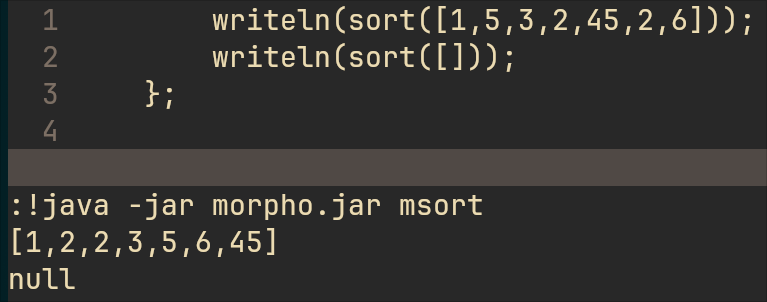
\includegraphics[scale=0.35]{msort.png}
	\end{center}
	Ath. að þegar morpho prentar tóma listann prentast "null" svo sort([]) 
	skilar í raun tóma listanum [].

\end{document}
